\documentclass[11pt]{article}
\usepackage[margin=0.68in]{geometry}
\usepackage{newtxtext,newtxmath}
\usepackage{booktabs,tabularx,multirow}
\usepackage{graphicx,xcolor}
\usepackage{amsmath}
\usepackage{microtype}
\usepackage{enumitem}
\usepackage{tikz}
\usetikzlibrary{arrows.meta,positioning,fit}
\usepackage[numbers,sort&compress]{natbib}
\usepackage[hidelinks]{hyperref}
\setlength{\parindent}{0pt}
\setlength{\parskip}{2.5pt}
\setlist{nosep,leftmargin=*}
\renewcommand{\baselinestretch}{1.0}
% This file is the only numerical-results file that should be edited after experiments.
% Existing pilot values are explicit; new Phase 3 values remain marked PENDING.
\newcommand{\PilotQRCNRMSE}{0.4127 $\pm$ 0.0062}
\newcommand{\PilotTCNNRMSE}{0.4167 $\pm$ 0.0020}
\newcommand{\FiveQNRMSE}{PENDING}
\newcommand{\TenQNRMSE}{PENDING}
\newcommand{\FifteenQNRMSE}{PENDING}
\newcommand{\IBMNRMSE}{PENDING}
\newcommand{\MNISTFiveAcc}{PENDING}
\newcommand{\MNISTTenAcc}{PENDING}
\newcommand{\MNISTFifteenAcc}{PENDING}


\title{\vspace{-1.4em}\textbf{Hardware-Portable Quantum Reservoir Computing for\\Regime-Sensitive VIX Volatility Forecasting}\vspace{-0.5em}}
\author{FraQTech -- Track A: Financial Volatility Prediction}
\date{}

\begin{document}
\maketitle
\vspace{-1.3em}
\begin{abstract}
We study whether a frozen quantum dynamical feature map can provide a selective forecasting benefit on regime-sensitive financial volatility while remaining executable on near-term hardware. Earlier pilot simulations across SPY, QQQ, and VIX found the clearest quantum-reservoir result on VIX: a continuous-variable QRC with a temporal convolutional readout attained NRMSE \PilotQRCNRMSE, compared with \PilotTCNNRMSE for a classical TCN. Phase 3 replaces the weak legacy gate model with a validation-selected temporal Ising QRC, benchmarks it against GARCH, HAR-RV, ESN, ridge, and TCN, and characterizes scaling over 5/10/15 qubits, finite shots, depolarizing and amplitude-damping noise, and physical QPU execution. We additionally implement the common MNIST expressivity benchmark and provide a fully reproducible qBraid workflow. Our claim is deliberately conditional: we test for a task-specific quantum benefit, not universal quantum advantage.
\end{abstract}

\section{Problem, data, and contributions}
Volatility forecasting is difficult because market dynamics are nonlinear, persistent, heavy-tailed, and subject to abrupt regime changes. Reservoir computing is a natural match: a fixed nonlinear dynamical system transforms an input history into a high-dimensional state trajectory, while only a lightweight readout is fitted \cite{jaeger2001echo}. QRC replaces the classical reservoir with driven quantum dynamics \cite{fujii2017harnessing,nakajima2019boosting}. Recent work has demonstrated few-atom feedback reservoirs, 108-qubit analog reservoirs, robust chaotic forecasting, and direct realized-volatility applications \cite{kornjaca2024large,zhu2025practical,ahmed2025robust,li2025volatility}. A recent unifying view emphasizes tuning the memory--nonlinearity balance rather than maximizing circuit complexity indiscriminately \cite{cindrak2026tradeoff}.

\textbf{Task.} From public daily VIX OHLC data (2015--2025), we compute log returns and a five-day rolling volatility proxy $v_t$. Given the previous 50 trading days, the primary task predicts $v_{t+1}$. A secondary task predicts whether $t+1$ lies above a causal rolling 80th-percentile high-volatility threshold, including explicit low-to-high transition recall. Splits are chronological 60/20/20; robust scaling is fitted on training data only. Architecture and hyperparameters are chosen by validation QLIKE, and the test set is evaluated once.

\textbf{Contributions.} (i) A hardware-portable, zero-trainable-quantum-parameter temporal Ising QRC with repeated angle encoding, fixed many-body dynamics, temporal multiplexing, and $Z/ZZ$ observables. (ii) A finance-appropriate comparison against GARCH(1,1), HAR-RV, ESN, ridge-lag, persistence, and TCN using RMSE, NRMSE, MAE, QLIKE, Mincer--Zarnowitz calibration, and prediction-level Diebold--Mariano tests \cite{bollerslev1986garch,corsi2009har,patton2011volatility,diebold1995comparing}. (iii) Reproducible 5/10/15-qubit, shot, noise, QPU, and MNIST studies on qBraid/IBM.

\section{Temporal Ising quantum reservoir}
For compressed temporal input $u_t$, each checkpoint applies data re-uploading followed by fixed non-commuting fields and Ising interactions,
\begin{align}
U_t &= \prod_{\nu=1}^{V} U_{\mathrm{res}}\,U_{\mathrm{enc}}(u_t),\\
U_{\mathrm{enc}}(u_t) &= \prod_i R_z(a_i^z u_t+b_i^z)R_y(a_i^y u_t+b_i^y),\\
U_{\mathrm{res}} &= \prod_{\ell=1}^{L}\left[\prod_{(i,j)\in E}R_{zz}(J_{ij}^{\ell})\prod_i R_z(h_{i,z}^{\ell})R_x(h_{i,x}^{\ell})\right].
\end{align}
All angles are fixed by a reported seed. The reservoir state is never variationally trained. At each virtual node we measure all $\langle Z_i\rangle$ and topology-edge $\langle Z_iZ_j\rangle$, plus four global summaries. Ridge is the primary readout because it most directly tests linear accessibility of reservoir information; a compact TCN is a secondary hybrid readout.

\begin{figure}[t]
\centering
\resizebox{\textwidth}{!}{%
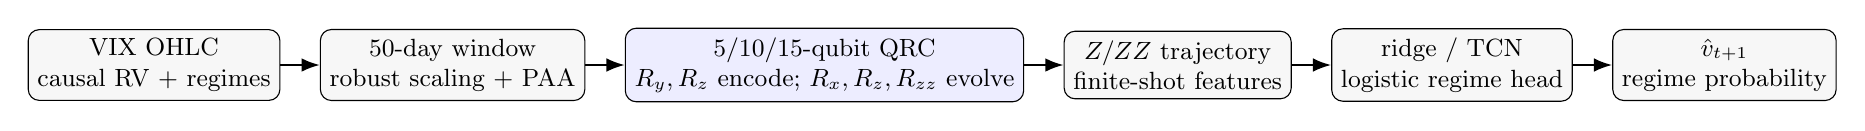
\begin{tikzpicture}[font=\small,node distance=5mm and 5mm,box/.style={draw,rounded corners,align=center,minimum height=8mm,fill=gray!6},arr/.style={-Latex,thick}]
\node[box] (data) {VIX OHLC\\causal RV + regimes};
\node[box,right=of data] (win) {50-day window\\robust scaling + PAA};
\node[box,right=of win,fill=blue!7] (qrc) {5/10/15-qubit QRC\\$R_y,R_z$ encode; $R_x,R_z,R_{zz}$ evolve};
\node[box,right=of qrc] (obs) {$Z/ZZ$ trajectory\\finite-shot features};
\node[box,right=of obs] (read) {ridge / TCN\\logistic regime head};
\node[box,right=of read] (out) {$\hat v_{t+1}$\\regime probability};
\draw[arr] (data)--(win);\draw[arr] (win)--(qrc);\draw[arr] (qrc)--(obs);\draw[arr] (obs)--(read);\draw[arr] (read)--(out);
\end{tikzpicture}%
}
\caption{End-to-end hybrid workflow. Only the classical readout is fitted. The same fixed circuit generator targets exact simulation, Qiskit Aer, IBM Runtime, and qBraid-managed gate QPUs.}
\label{fig:pipeline}
\end{figure}

\textbf{Selection and controls.} On validation only, a 5-qubit search varies topology, 4/6/8 temporal bins, 1/2 virtual nodes, 1/2 reservoir layers, re-uploading, interaction scale, and ridge penalty. We then freeze the winning design before testing. Controls include Z-only features, no re-uploading, line topology, ESN states, raw windows, and a matched-dimensional nonlinear random projection. These distinguish a useful quantum trajectory from a large arbitrary feature expansion.

\section{Experimental protocol and platform use}
Table~\ref{tab:matrix} summarizes the final matrix. Exact statevectors establish an ideal reference; Qiskit Aer adds 256/1024/4096-shot sampling and explicit depolarizing/amplitude-damping channels. For hardware, a shallower six-checkpoint, five-qubit ring reservoir is transpiled to the selected backend. IBM EstimatorV2 directly evaluates the $Z/ZZ$ operator set, with optimization level 3, resilience level 1, and XY4 dynamical decoupling. Every result records logical/transpiled depth, two-qubit gates, shots, runtime, backend, and job IDs. An optional qBraid-managed second gate QPU provides cross-platform validation. We do not use annealing hardware because the computation is driven temporal dynamics rather than QUBO optimization.

\begin{table}[t]
\centering\small
\caption{Frozen Phase 3 evaluation matrix.}
\label{tab:matrix}
\begin{tabularx}{\textwidth}{lXl}
\toprule
Block & Configurations & Outputs\\
\midrule
Classical & persistence, GARCH, HAR-RV, ridge, ESN, TCN; 5 seeds & NRMSE, QLIKE, MZ, runtime\\
QRC scaling & 5/10/15 qubits; ridge and TCN; 3 seeds & accuracy/resource curves\\
Measurement/noise & 256/1024/4096 shots; depolarizing and damping; 3 seeds & degradation and feature drift\\
Hardware & IBM 5q targeted test subset; optional second qBraid gate QPU & depth, gates, shots, jobs, metrics\\
Regimes & raw, ESN, and QRC features & macro-F1, AUROC, Brier, transition recall\\
MNIST & fixed 2000/500 subset; 5/10/15 qubits & accuracy, macro-F1, runtime\\
\bottomrule
\end{tabularx}
\end{table}

The common MNIST benchmark resizes digits to $8\times8$ and interprets rows as an eight-step sequence through the same reservoir family, followed by multinomial logistic regression. This is an expressivity check, not evidence for financial quantum advantage.

\section{Results and analysis plan}
The prior VIX pilot provides the starting point in Table~\ref{tab:pilot}. It motivates VIX as the primary case but does not establish a qubit-hardware benefit because the winning encoder was a continuous-variable moment simulator. The new gate-QRC must therefore be evaluated independently.

\begin{table}[t]
\centering\small
\caption{Completed pilot evidence and Phase 3 result slots. New values are generated from raw JSON and prediction CSV artifacts.}
\label{tab:pilot}
\begin{tabular}{lccc}
\toprule
Model & Qubits & VIX NRMSE $\downarrow$ & Status\\
\midrule
Classical TCN & 0 & \PilotTCNNRMSE & completed pilot\\
CV-QRC + TCN & modes & \PilotQRCNRMSE & completed pilot\\
Temporal Ising QRC + ridge & 5 & \FiveQNRMSE & pending execution\\
Temporal Ising QRC + ridge & 10 & \TenQNRMSE & pending execution\\
Temporal Ising QRC + ridge & 15 & \FifteenQNRMSE & pending execution\\
IBM QPU subset & 5 & \IBMNRMSE & pending execution\\
\bottomrule
\end{tabular}
\end{table}
\IfFileExists{auto_results_table.tex}{% Generated by scripts/aggregate_phase3.py after experiments.
}{}

The principal statistical question is whether the selected gate-QRC improves QLIKE or NRMSE relative to ESN/ridge/TCN across seeds and whether any improvement survives matched-dimensional random features. Prediction-level Diebold--Mariano tests assess loss differences. Noise results will report both forecast degradation and feature drift from the exact statevector reference. Hardware is interpreted through the chain exact $\rightarrow$ finite-shot $\rightarrow$ noisy simulator $\rightarrow$ QPU; a competitive or gracefully degraded QPU result is meaningful even if it does not beat the best classical TCN.

\section{Stakeholder value, limitations, and reproducibility}
A useful volatility forecast can support risk limits, market-making inventory, derivatives hedging, and regime-aware allocation. The practical contribution is not merely a small accuracy change: it is a transparent decision boundary describing when a fixed quantum feature service is worth its circuit and shot cost.

Limitations are explicit. Exact simulation scales exponentially; the QPU test is a targeted subset; market data and volatility proxies are imperfect; the TCN may account for much of the pilot gain; and one dataset cannot support a universal advantage claim. The final claim will therefore be one of \emph{selective quantum benefit} only if gate-QRC gains survive ablations, noise, and fair classical comparison.

The submission includes project-relative code, a frozen data manifest/checksum, one-command smoke tests, prediction-level outputs, qBraid/IBM adapters, a qBraid Skill, and a complete README. Judges can reproduce simulator headlines without credentials and can re-run QPU jobs after configuring their own authorized account. Generative AI was used for code/documentation assistance; all executed results and scientific claims are produced and verified by the team.

\begin{thebibliography}{16}\small
\bibitem{fujii2017harnessing} K. Fujii and K. Nakajima, ``Harnessing disordered-ensemble quantum dynamics for machine learning,'' \emph{Phys. Rev. Applied}, 8, 024030, 2017.
\bibitem{nakajima2019boosting} K. Nakajima et al., ``Boosting computational power through spatial multiplexing in quantum reservoir computing,'' \emph{Phys. Rev. Applied}, 11, 034021, 2019.
\bibitem{kornjaca2024large} M. Kornjaca et al., ``Large-scale quantum reservoir learning with an analog quantum computer,'' arXiv:2407.02553, 2024.
\bibitem{zhu2025practical} C. Zhu et al., ``Practical few-atom quantum reservoir computing,'' \emph{Phys. Rev. Research}, 7, 023290, 2025.
\bibitem{ahmed2025robust} O. Ahmed, F. Tennie, and L. Magri, ``Robust quantum reservoir computers for forecasting chaotic dynamics,'' \emph{Proc. R. Soc. A}, 481, 20250550, 2025.
\bibitem{li2025volatility} Q. Li et al., ``Quantum Reservoir Computing for Realized Volatility Forecasting,'' arXiv:2505.13933, 2025.
\bibitem{hou2026high} Y. Hou et al., ``High-Accuracy Temporal Prediction via Experimental Quantum Reservoir Computing in Correlated Spins,'' arXiv:2508.12383, 2025.
\bibitem{cindrak2026tradeoff} S. Cindrak et al., ``Memory-Nonlinearity Trade-off across Quantum Reservoir Computing Frameworks,'' arXiv:2603.21371, 2026.
\bibitem{jaeger2001echo} H. Jaeger, ``The echo state approach to analysing and training recurrent neural networks,'' GMD Report 148, 2001.
\bibitem{bollerslev1986garch} T. Bollerslev, ``Generalized autoregressive conditional heteroskedasticity,'' \emph{J. Econometrics}, 31, 307--327, 1986.
\bibitem{corsi2009har} F. Corsi, ``A simple approximate long-memory model of realized volatility,'' \emph{J. Financial Econometrics}, 7, 174--196, 2009.
\bibitem{patton2011volatility} A. J. Patton, ``Volatility forecast comparison using imperfect volatility proxies,'' \emph{J. Econometrics}, 160, 246--256, 2011.
\bibitem{diebold1995comparing} F. X. Diebold and R. S. Mariano, ``Comparing predictive accuracy,'' \emph{J. Business and Economic Statistics}, 13, 253--263, 1995.
\bibitem{qiskit2024} A. Javadi-Abhari et al., ``Quantum computing with Qiskit,'' arXiv:2405.08810, 2024.
\bibitem{qbraid2026} R. J. Hill et al., ``qBraid-SDK: Platform-agnostic quantum runtime framework,'' v0.12.1, 2026.
\end{thebibliography}
\end{document}
